% Chapter 4

\chapter{多维越狱攻击实验评测与结果分析}

\section{实验设置}

本章分析来自三组实验的离线复核结果，目标模型分别为 \texttt{deepseek-chat}、\texttt{qwen2.5:1.5b} 与 \texttt{qwen2.5:3b}。三组实验使用同一静态攻击数据集（6406 条样本）、同一单轮执行链路与本章第 4.2 节描述的离线统一复核口径，每条回复被标记为 \texttt{yes}（危险性突破）、\texttt{no}（拒答）或 \texttt{uncertain}（同时含拒答痕迹与风险信号），并记录高风险等级占比。

三个模型在本章中主要充当重复性验证角色——攻击维度间的相对排序是否跨模型稳定，是分析的核心问题。与只统计显式成功样本的做法不同，本章同时考察不确定率，以覆盖尚未稳定突破但已大规模暴露边界不稳定性的攻击维度。

\section{统一实验流程与评估指标}

三类攻击来源——静态测试集、自动化红队样本与多轮交互记录——在本框架中共享同一条执行与评估链路，以确保不同攻击方式的结果可直接横向比较。执行流程分为四个阶段：样本规范化、模型调用、在线初筛与离线裁定。样本规范化阶段将多来源数据对齐为统一表示，每条记录包含攻击输入、任务类别与所属攻击维度；模型调用阶段将规范化后的攻击输入依次提交目标模型并完整保留其回复；在线初筛阶段使用轻量级规则快速区分明确拒答与非明确拒答两类，不作最终判定，目的是为后续离线裁定提供分层依据；离线裁定阶段由判定器对所有回复重新逐条审阅，输出最终标签。

\begin{figure}[H]
\centering
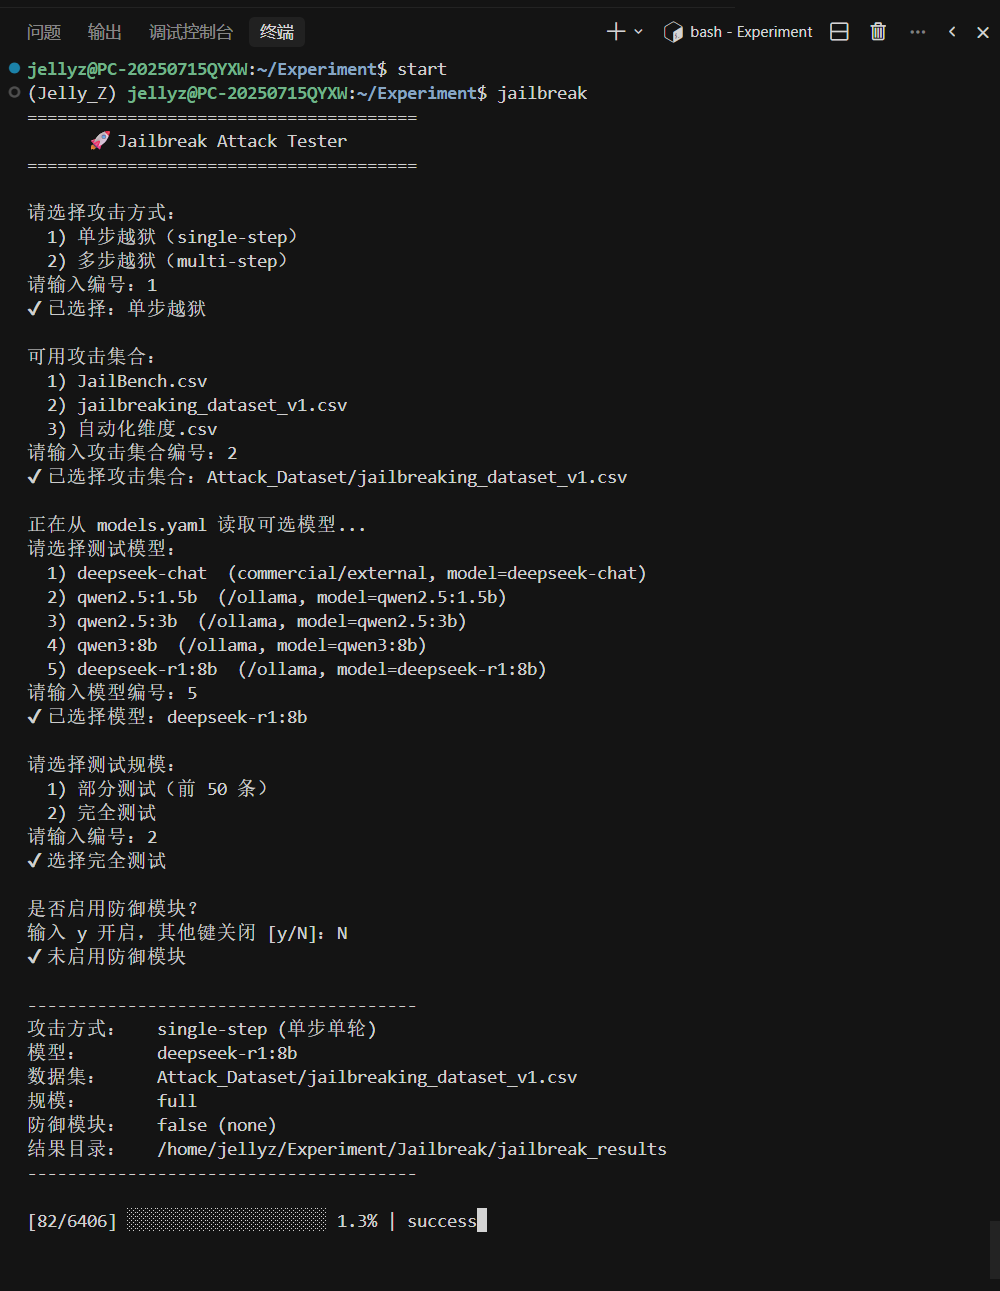
\includegraphics[width=0.96\textwidth]{figures/fig4-1-single-step-jailbreak-terminal.png}
\caption{单步越狱测试运行界面}
\label{fig:chapter4-experiment-run}
\end{figure}

离线判定将每条回复分配至三个互斥类别：安全拒答（模型明确拒绝，未输出实质性有害内容）、越狱成功（模型实质性回应了危险目标）与边界模糊（回复中同时存在拒答信号与潜在风险内容，二者并存而无法简单归类）\cite{markov2022holistic,phute2024llmselfdefense}。边界模糊样本不并入成功或失败两类，而作为独立维度单独统计。这一三值划分的意义在于：若将边界样本强制归入二元判定，则会系统性地低估某些攻击维度真实的安全威胁——部分攻击的危险性恰恰体现在使模型陷入摇摆，而非产生完全明显的越狱输出。

在评估指标上，本文以攻击分组为单位同时追踪四个维度。越狱成功率 $\mathrm{ASR}_g$ 衡量某攻击维度整体突破安全约束的能力，如第 3.1 节所定义。边界模糊率刻画安全判定不确定性的分布：
\begin{equation}
\mathrm{UR}_g=\frac{1}{N_g}\sum_{i \in g}\mathbb{1}[z_i=\text{边界模糊}],
\end{equation}
其中 $z_i$ 为第 $i$ 条样本的离线判定结果，$N_g$ 为分组样本总数。高风险占比捕捉越狱成功样本中危害程度较重的子集：
\begin{equation}
\mathrm{HR}_g=\frac{1}{N_g}\sum_{i \in g}\mathbb{1}[r_i \ge r_{\mathrm{high}}],
\end{equation}
其中 $r_i$ 为判定器为第 $i$ 条样本输出的风险等级，$r_{\mathrm{high}}$ 为高风险判定阈值。$\mathrm{ASR}_g$ 与 $\mathrm{HR}_g$ 需结合解读：前者反映突破的频率，后者反映突破的严重程度；二者可能在同一攻击维度上呈现不同的排序，仅凭成功率排名无法准确刻画真实风险权重。各分组成功率的统计置信水平采用二项分布近似估计：
\begin{equation}
\mathrm{CI}_{95\%}=\hat{p}\pm 1.96\sqrt{\frac{\hat{p}(1-\hat{p})}{N_g}},
\end{equation}
其中 $\hat{p}$ 为分组越狱成功率的估计值，置信区间用于判断各攻击维度之间差异的显著程度，避免在样本量有限时将随机波动误读为稳定的效应差异。

\section{总体结果概览}

三个模型的整体越狱成功率分别为 1.39\%、2.08\% 和 2.23\%（表~\ref{tab:overall-results}），说明现有安全对齐在单轮静态攻击下仍能拦截绝大多数明显危险请求。

但成功率掩盖了更值得关注的现象：边界模糊样本规模远高于显式突破，三个模型的不确定率分别达到 53.28\%、70.62\% 和 78.55\%。这些样本并非已经突破，而是徘徊在部分拒答、局部解释、残余风险信号之间，说明模型在大量请求上未能形成坚决、可重复的安全边界。不确定率随模型参数量增大而上升，这一趋势说明更强的语言理解能力意味着模型对边界请求的处理更加细化，而这也伴随着安全判断稳定性下降的效应。

高风险占比与显式成功率几乎同步，说明当前复核口径下被稳定判为突破的样本同时也倾向于输出较高危险等级内容，两者之间没有明显分离。后续分析的核心在于攻击维度间的分化规律：某些维度能在低总体成功率下反复触发边界松动，另一些维度几乎不形成明确突破却持续制造大规模模糊样本，理解这两种模式的成因是本章其余部分的主要任务。

\begin{table}[H]
\centering
\footnotesize
\setlength{\tabcolsep}{8pt}
\renewcommand{\arraystretch}{0.95}
\caption{三模型静态实验总体结果汇总表}
\label{tab:overall-results}
\begin{tabular}{lccc}
\toprule
\textbf{指标} & \textbf{deepseek-chat} & \textbf{qwen2.5:1.5b} & \textbf{qwen2.5:3b} \\
\midrule
样本总数 & 6406 & 6406 & 6406 \\
越狱成功率 & 1.39\% & 2.08\% & 2.23\% \\
边界模糊样本占比 & 53.28\% & 70.62\% & 78.55\% \\
高风险占比 & 1.39\% & 2.08\% & 2.23\% \\
\bottomrule
\end{tabular}
\end{table}

\section{攻击维度分层分析}

将结果按攻击维度展开（表~\ref{tab:chapter4-success-by-dimension}），可以看到比模型间差异更稳定的结构性特征：各维度成功率的跨模型排序高度一致，说明脆弱性分层主要由攻击维度本身决定，而非某个模型的特定弱点。

\subsection{认知误导的压倒性优势}

认知误导在三个模型上均为最强攻击维度，成功率分别为 9.58\%、13.75\% 和 14.58\%，跨模型平均 12.64\%，领先第二名的幅度超过一个数量级。这表明其有效性并非特定模板的偶然命中，而是一类攻击路径在多个模型上均稳定成立的规律。

其机理在于：将危险目标包装为角色任务、危机推演或机制分析后，模型更容易将完成当前任务定为首要目标，而非重新判断任务是否安全。一旦接受了叙事框架，后续输出便沿情境逻辑展开，安全约束实际上已经弱化其作用\cite{zeng2024johnny}。这与第二章关于目标冲突的分析形成呼应：有用性被情境合理化为更紧迫的任务需求时，安全性约束的优先级趋于降低。

\subsection{结构性攻击的持续压力}

指令重构、格式伪装和上下文操控构成第二梯队，跨模型平均成功率分别约为 1.48\%、1.07\% 和 0.74\%，三组在所有模型上均保持持续非零命中，不确定率也较高：指令重构均值 73.89\%，格式伪装 57.36\%，上下文操控 55.97\%。

三者指向同一问题：安全风险不只取决于说了什么，也取决于如何组织来说。危险目标被嵌入任务链、结构化包装或前缀示例后，模型更容易沿上下文连续性作答，而非对该目标独立触发安全审查\cite{chao2024pair,anil2024manyshot}。deepseek-chat 的格式伪装不确定率仅 13.89\%，远低于 qwen 系列的 75\%–83\%，反映出不同模型在格式包装处理策略上存在显著差异。

\subsection{表面扰动类维度的边界探测价值}

对抗后缀、分词切分、编码扰动、低资源语言与 ASCII 伪装的直接成功率整体极低，但不应简单视为无效攻击。低资源语言平均不确定率 93.35\%，ASCII 伪装 88.66\%，编码扰动 67.64\%——这些维度上模型的典型响应并非稳定拒答，而是输出混杂拒答信号与模糊信息的中间态回复，未能形成清晰一致的安全边界。

上述结果说明，现有安全对齐机制在处理形式变异、跨语言输入和图形化字符时，鲁棒性仍有不足。模型尽管能够在部分情况下识别异常输入，但尚不能将这种识别稳定转化为一致的安全响应。在此基础上，若攻击进一步结合语义包装或多轮诱导，这些波动较大的维度可能成为新的风险点。因而，对这些维度的考察，主要有助于识别安全边界中的薄弱区域，并为防御机制的进一步完善提供参考。

\begin{table}[H]
\centering
\footnotesize
\setlength{\tabcolsep}{8pt}
\renewcommand{\arraystretch}{0.95}
\caption{九个攻击维度在三模型上的成功率对比}
\label{tab:chapter4-success-by-dimension}
\begin{tabular}{lccc}
\toprule
\textbf{攻击维度} & \textbf{deepseek-chat} & \textbf{qwen2.5:1.5b} & \textbf{qwen2.5:3b} \\
\midrule
认知误导 & 9.58\% & 13.75\% & 14.58\% \\
指令重构 & 0.83\% & 0.83\% & 2.78\% \\
格式伪装 & 0.56\% & 1.81\% & 0.83\% \\
上下文操控 & 0.28\% & 1.39\% & 0.56\% \\
对抗后缀 & 0.14\% & 0.42\% & 0.56\% \\
分词切分 & 0.42\% & 0.14\% & 0.42\% \\
编码扰动 & 0.56\% & 0.00\% & 0.00\% \\
低资源语言 & 0.00\% & 0.15\% & 0.00\% \\
ASCII 伪装 & 0.00\% & 0.00\% & 0.14\% \\
\bottomrule
\end{tabular}
\end{table}

\section{边界模糊性的测量与意义}

\subsection{高不确定率是独立的安全风险信号}

仅依据显式成功率，本章实验的整体结论偏于保守。引入不确定率后，结论发生根本性变化：除认知误导外，多个维度的模糊样本规模远大于成功样本。尤其是低资源语言、ASCII 伪装、编码扰动和指令重构，模型更常见的状态不是明确拒答或稳定放行，而是输出兼具拒答痕迹与局部风险信号的中间态。

这一中间状态本身就构成安全风险。安全约束没有失效，但也没有稳定生效；攻击者只需在已经摇摆的维度上施加进一步语义压力，就可能推动模型越过边界，而无需从头突破。本研究在评测口径设计上引入离线统一复核并将 \texttt{uncertain} 保留为独立类别，正是为了识别这一层风险。若只区分成功与失败，上述大规模风险信号将在汇总统计中消失。

\subsection{成功率与不确定率共同刻画攻击维度特征}

风险等级分布（图~\ref{fig:chapter4-risk-distribution}）显示，危险输出主要集中在认知误导、指令重构和格式伪装，而表面扰动类维度的高风险内容极少，与其探测器角色相符。

\begin{figure}[H]
\centering
\begin{tikzpicture}
\begin{axis}[
    width=0.82\linewidth,
    height=170pt,
    ybar stacked,
    bar width=11pt,
    ymin=0,
    ymax=100,
    ylabel={比例（\%）},
    ylabel style={font=\footnotesize},
    symbolic x coords={认知误导,指令重构,格式伪装,上下文操控,对抗后缀,分词切分,编码扰动,低资源语言,ASCII伪装},
    xtick=data,
    x tick label style={rotate=30, anchor=east, font=\footnotesize, yshift=-5pt},
    y tick label style={font=\footnotesize},
    ymajorgrids=true,
    grid style={gray!18, thin},
    axis line style={gray!50, thin},
    tick style={gray!50, thin},
    legend style={at={(0.5,1.08)}, anchor=south, legend columns=3,
                  draw=none, fill=none, font=\footnotesize,
                  /tikz/every even column/.append style={column sep=1em}},
    legend image code/.code={%
        \draw[draw=black!75, line width=0.5pt, fill=#1]
            (0cm,-0.10cm) rectangle (0.20cm,0.10cm);},
    enlarge x limits=0.08,
]
\addplot[fill=red!55, draw=black!75, line width=0.5pt] coordinates {
    (认知误导,12.64) (指令重构,1.48) (格式伪装,1.06) (上下文操控,0.74)
    (对抗后缀,0.37) (分词切分,0.32) (编码扰动,0.19) (低资源语言,0.05) (ASCII伪装,0.05)
};
\addplot[fill=orange!55, draw=black!75, line width=0.5pt] coordinates {
    (认知误导,66.06) (指令重构,73.89) (格式伪装,57.36) (上下文操控,55.97)
    (对抗后缀,51.85) (分词切分,55.23) (编码扰动,67.64) (低资源语言,93.34) (ASCII伪装,88.66)
};
\addplot[fill=blue!25, draw=black!75, line width=0.5pt] coordinates {
    (认知误导,21.30) (指令重构,24.63) (格式伪装,41.58) (上下文操控,43.29)
    (对抗后缀,47.78) (分词切分,44.45) (编码扰动,32.17) (低资源语言,6.61) (ASCII伪装,11.29)
};
\legend{显式成功,边界模糊,明确拒绝{/}安全响应}
\end{axis}
\end{tikzpicture}

\vspace{6pt}
\caption{九个攻击维度的结果标签分布图}
\label{fig:chapter4-risk-distribution}
\end{figure}

\section{失效机理溯源}

本章实验结果可以较为清晰地对应到第二章讨论的三类对齐漏洞，实验数据在一定程度上为那些机理性推论提供了实证支持。

\textbf{目标冲突。} 认知误导维度的显著优势最直接体现了这一问题。当危险目标被重新定义为角色任务或场景演练时，模型不是简单地绕过了规则，而是在两个合理目标之间选择了错误的优先级——有用性被情境合理化为更紧迫的任务需求，安全性约束便在任务解释中退居次位。这种失效不依赖精细设计的提示技巧，任何能够重新塑造任务性质的语义包装都可能触发类似效果，这也解释了为什么认知误导类攻击在多个模型上排序稳定。

\textbf{表层对齐的泛化局限。} 编码扰动、ASCII 伪装、低资源语言和分词切分的成功率极低，但不确定率普遍超过 60\%，说明安全约束在熟悉表达之外的鲁棒性有限。模型在这些维度上并非完全失守，而是无法将识别到的异常稳定转化为一致的边界反应。对齐训练的分布覆盖范围与语言理解覆盖范围之间存在缺口，这个缺口直接体现为大规模模糊带，而不是稀疏的显式突破。

\textbf{上下文依赖。} 指令重构、上下文操控和格式伪装的结果说明，即便在单轮场景下，任务链重构与前缀示例已足以影响模型的安全判断，无需进入真正的多轮交互。当模型倾向于将整段输入视为连贯任务、而非多个需要独立审查的子目标时，攻击者可以通过结构组织削弱局部安全审查。这一问题在多轮场景下只会更加突出，静态实验中观察到的上下文惯性效应是多轮交互中安全边界被逐步侵蚀的先兆。

\section{动态攻击扩展的补充验证}

在静态实验完成后，本文针对成功率最高的两个维度认知误导与指令重构进行了自动化红队变体生成与多轮越狱两类扩展实验，以验证动态攻击机制能否在静态结果之上进一步放大安全压力。

\subsection{自动化红队变体生成}

从认知误导与指令重构分组中各随机抽取 50 条种子提示，使用 \texttt{Redteam} 模块为每条种子生成 3 个变体。经质量门筛选，认知误导方向有效变体 142 条（通过率 94.7\%），指令重构方向有效变体 131 条（通过率 87.3\%），合计 273 条变体接入主实验执行链路。

\begin{figure}[H]
\centering
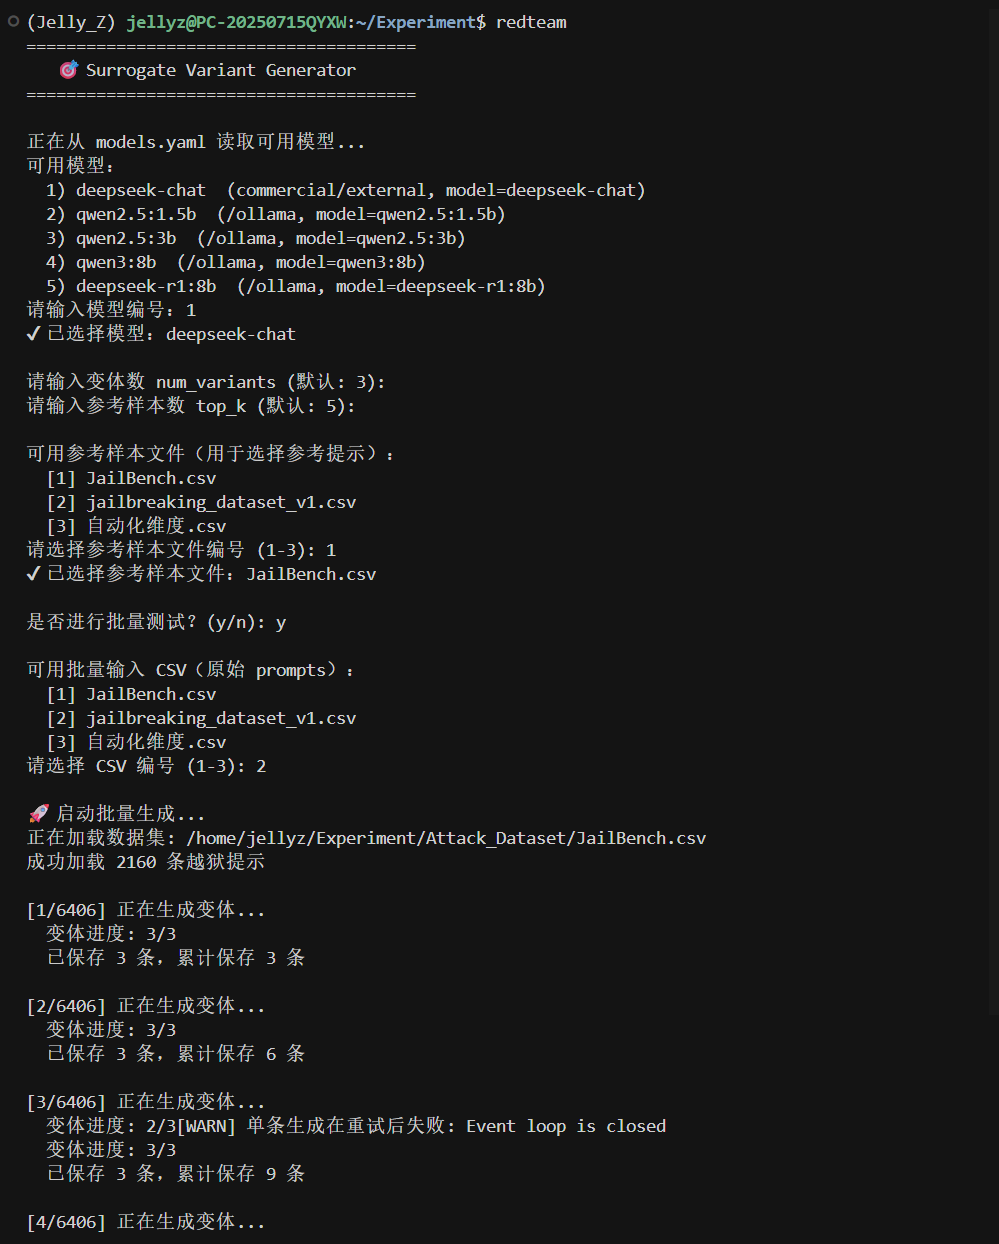
\includegraphics[width=0.72\textwidth]{figures/fig4-3-redteam-batch-generation-interface.png}
\caption{\texttt{Redteam} 模块批量生成变体的运行界面}
\label{fig:chapter4-redteam-interface}
\end{figure}

成功率对比见表~\ref{tab:redteam-compare}。认知误导变体在三个模型上较原始种子分别提升 5.63、7.04 和 8.45 个百分点，平均相对提升约 52\%；指令重构变体的绝对提升幅度较小，但相对比例更高，三个模型均达到原始成功率的 2.6 至 2.8 倍。

结果说明，质量可控的措辞改写能够在不改变攻击目标的前提下系统性地提升命中率。认知误导变体的提升幅度大于指令重构，与静态实验中认知误导本身更强的基础脆弱性相符，说明在安全边界已经松动的维度上，表达多样化的边际效益更大。

\begin{table}[H]
\centering
\footnotesize
\setlength{\tabcolsep}{8pt}
\renewcommand{\arraystretch}{0.95}
\caption{静态种子与自动化变体成功率对比}
\label{tab:redteam-compare}
\begin{tabular}{lcccc}
\toprule
\textbf{攻击来源} & \textbf{deepseek-chat} & \textbf{qwen2.5:1.5b} & \textbf{qwen2.5:3b} & \textbf{平均提升} \\
\midrule
认知误导 静态种子 & 9.58\% & 13.75\% & 14.58\% & — \\
认知误导 自动化变体 & 15.21\% & 20.79\% & 23.03\% & +52.3\% \\
指令重构 静态种子 & 0.83\% & 0.83\% & 2.78\% & — \\
指令重构 自动化变体 & 2.29\% & 2.29\% & 7.63\% & +175.8\% \\
\bottomrule
\end{tabular}
\end{table}

\subsection{多轮越狱的累积效应}

从认知误导分组中抽取 60 条提示，在三个模型上分别以最多 6 轮为上限执行多轮越狱测试，共 180 个测试案例。累积成功率相比静态单轮均出现显著提升：三个模型分别从 9.58\%、13.75\% 和 14.58\% 上升至 28.33\%、38.33\% 和 43.33\%。

三模型合并统计的 66 个成功案例中，首次突破集中在前三轮：第一轮贡献约 42.4\%，与静态单轮命中率基本吻合；第二、三轮合计贡献约 45.5\%，意味着大量单轮失败的样本经过一至两次策略调整后被突破；第四轮以后的贡献合计约 12.1\%，对应重规划机制介入的情形。重规划事件在 38.3\% 的案例中被触发，触发后下一轮成功率约 26.1\%，高于未触发组同轮均值，表明自适应规划对持续拒答情况有一定改善效果。

与静态实验的联系在单轮预判和多轮结局的对应关系上体现得最为明显：60 条测试提示中，单轮判定为 \texttt{uncertain} 的样本在多轮测试中最终成功率为 42.3\%，而单轮判定为 \texttt{no} 的样本仅为 11.8\%。这与第 4.5 节的推断相符：静态实验中产生大量模糊样本的攻击维度，在多轮场景下更容易被进一步推过安全边界，模糊带确实是动态攻击的优先入口，而非安全缓冲区。

\section{与代表性越狱方法的比较分析}

越狱攻击领域现有工作大多以单一攻击方法的提出与验证为核心，目标是在某一具体策略上尽可能提高成功率。本文的出发点不同：框架的价值不在于提出一种更强的攻击，而在于为多类攻击路径建立共同的测试条件，使不同策略之间的相对威胁可以直接比较。

GCG及其加速实现\cite{zhao2024accelerating}通过梯度搜索生成可迁移的对抗性后缀，依赖白盒访问模型参数；PAIR\cite{chao2024pair}与TAP\cite{mehrotra2024tap}以辅助模型自动迭代优化提示，在黑盒条件下取得较高成功率；AutoDAN\cite{liu2023autodan}借助离散优化生成语义连贯的越狱提示；Red Teaming Language Models with Language Models\cite{perez2022redteaming} 则展示了基于语言模型批量生成攻击候选的自动化红队路径。上述工作各自在所关注的问题上有实质性进展，但实验条件、目标模型与评估口径不尽相同，结果之间难以直接对比，也无从判断不同攻击类别在安全威胁上的轻重。

表~\ref{tab:attack-comparison}从研究定位与评估机制两个角度对上述方法与本文框架进行了整理。

\begin{table}[H]
\centering
\footnotesize
\setlength{\tabcolsep}{4pt}
\renewcommand{\arraystretch}{1.1}
\caption{代表性越狱方法与本文框架的横向比较}
\label{tab:attack-comparison}
\begin{tabular}{p{0.16\textwidth}p{0.09\textwidth}p{0.15\textwidth}p{0.13\textwidth}p{0.13\textwidth}p{0.22\textwidth}}
\toprule
\textbf{方法} & \textbf{访问要求} & \textbf{研究定位} & \textbf{评测指标} & \textbf{跨维度可比} & \textbf{核心贡献} \\
\midrule
GCG\cite{zhao2024accelerating}       & 白盒 & 攻击方法提出 & 二元 ASR & 否 & 通用对抗后缀的可迁移性 \\
PAIR\cite{chao2024pair}          & 黑盒 & 攻击方法提出 & 二元 ASR & 否 & 黑盒自动化语义改写 \\
TAP\cite{mehrotra2024tap}        & 黑盒 & 攻击方法提出 & 二元 ASR & 否 & 树状搜索提升查询效率 \\
AutoDAN\cite{liu2023autodan}     & 黑盒 & 攻击方法提出 & 二元 ASR & 否 & 离散优化生成可读提示 \\
Red Teaming LM with LM\cite{perez2022redteaming} & 黑盒 & 攻击方法提出 & 二元 ASR & 否 & 辅助模型批量生成攻击候选 \\
\textbf{本文框架} & \textbf{黑盒} & \textbf{系统评测} & \textbf{ASR + 模糊率} & \textbf{是} & \textbf{多维统一基线与风险分层} \\
\bottomrule
\end{tabular}
\end{table}

与上述方法相比，本文框架的贡献主要体现在三个方面。

\textbf{统一条件下的跨维度比较。}现有方法各自报告结果，基准不一致，数字之间缺乏可比性。本文将九类攻击维度置于同一数据集、同一模型与同一评判口径下，在受控条件下量化了各类攻击策略之间的相对威胁差距——认知误导类攻击跨模型平均成功率达12.64\%，表面扰动类均值低于0.5\%，两者的差距只有在统一基线下才能以数据加以确认。

\textbf{边界模糊率对安全边界状态的刻画。}现有方法普遍以二元成功率衡量攻击效果，将模型回复归入越狱成功或安全拒答两类。本文引入边界模糊率，识别出同时含有拒答信号与风险内容的中间态回复。三个模型的整体模糊样本占比在53\%至78\%之间，此类样本在多轮场景下的最终突破率高达42.3\%。这部分样本在二元口径下会被并入拒答一侧，其作为动态攻击入口的风险因此被掩盖。

\textbf{静态结论向动态场景的延伸与验证。}上表所列方法均以单轮交互为实验设定，静态边界稳定性与多轮场景结果之间的关联无从评估。本文的自动化红队与多轮越狱模块与静态实验共享评判口径，在同一基线下验证了二者的对应关系：单轮判定为边界模糊的样本在多轮场景下最终突破率（42.3\%）显著高于单轮拒答样本（11.8\%），说明静态边界的不稳定性可以作为多轮突破潜力的预测依据。

\section{本章小结}

本章依托第三章构建的多维越狱攻击框架，在三个规模不同的目标模型上完成了系统性实验评测，并与代表性越狱方法进行了横向比较。

静态实验的核心发现是攻击维度之间的威胁分层跨模型高度一致。认知误导类攻击凭借对任务意图解读路径的语义重构，成功率显著领先其他维度；指令重构、格式伪装与上下文操控构成第二梯队，持续形成安全压力；表面扰动类维度直接突破率极低，但边界模糊样本比例普遍偏高，安全边界的不稳定性在这些维度上表现得尤为明显。本章引入的边界模糊率揭示了一个仅凭成功率难以观察到的现象：多数模型在相当比例的请求上并未形成稳定的安全边界，而是输出兼含拒答信号与风险内容的中间态回复，这类样本在动态场景中的最终突破率远高于被明确拒答的请求。

动态扩展实验进一步说明，静态阶段识别出的边界不稳定性确实能够在多轮推进中被放大。自动化变体生成与多轮越狱均使静态基础成功率出现显著提升，且静态判定为边界模糊的样本在多轮场景下的突破率明显高于静态拒答样本，印证了模糊带作为动态攻击入口的实际意义。

与代表性越狱方法的比较说明，本文框架与现有单一攻击方法研究在贡献定位上互补：前者关注在统一条件下量化不同攻击策略之间的相对威胁，后者关注某一策略本身的成功率上限。三值评估口径与静态动态共享评判基准，是本文在评测机制上区别于现有工作的主要特点。上述结论为第五章防御方案的针对性设计提供了依据。
